\begin{frame}
  \begin{center}
    \LARGE <<Латинский квадрат>>
  \end{center}
  \begin{center}
      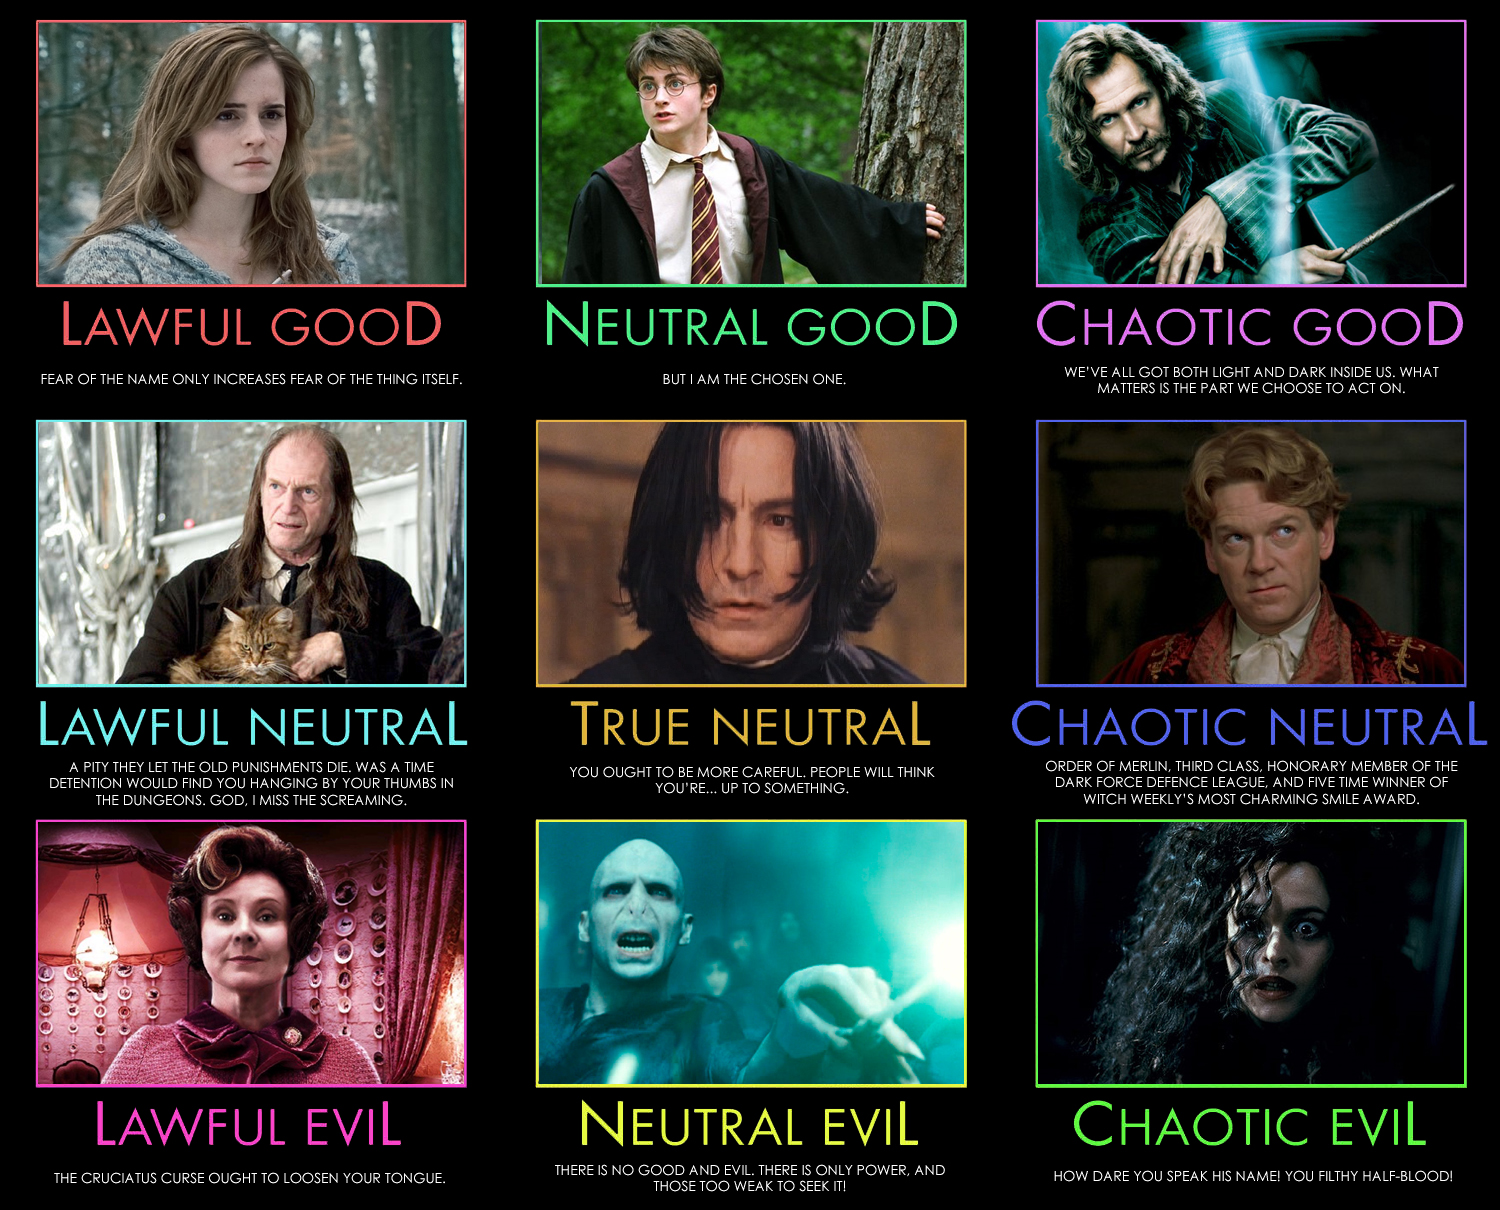
\includegraphics[width=5cm]{memes/h-meme.jpg}
  \end{center}
  \begin{itemize}
  \item Идея задачи --- Михаил Тихомиров, МФТИ
  \item Разработка задачи --- Николай Будин, ИТМО
  \end{itemize}
\end{frame}

\begin{frame}{Постановка задачи}

  \begin{itemize}
  \item Дана матрица $n \times m$.
  \item Нужно найти количество подматриц, которые являются латинскими квадратами.
  \item Латинский квадрат~--- матрица $k \times k$, в которой ровно $k$ различных элементов и в каждой строке и каждом столбце элементы не повторяются.
  \end{itemize}
  
\end{frame}

\begin{frame}{Решение за $\O(n ^ 5)$ (9 баллов)}
  \begin{itemize}
  \item Переберем подматрицу, являющуюся квадратом.
  \item Проверим, что подматрица является латинским квадратом за её размер.
  \item В зависимости от используемых для проверки структур данных, асимптотика может дополнительно умножиться на логарифм.
  \end{itemize}
\end{frame}

\begin{frame}{Решение за $\O(n ^ 4)$ (19~баллов)}
  Сделаем наблюдение:
  
  \begin{itemize}
  \item Квадратная подматрица является латинским квадратом, если:
  \begin{itemize}
  \item В каждой строке и каждом столбце все элементы различны,
  \item Количество различных элементов в подматрице равно длине её стороны.
  \end{itemize}
  \end{itemize}
\end{frame}

\begin{frame}{Решение за $\O(n ^ 4)$ (19~баллов)}
  \vspace{-0.7em}
  \begin{itemize}
  \item Зафиксируем верхний левый угол латинского квадрата.
  \item Будем перебирать длину стороны квадрата в порядке возрастания.
  \item При увеличении стороны на $1$, добавляем новые элементы и проверяем, что не появилось дубликатов в какой-то строке или столбце.
    Также поддерживаем число различных в текущем квадрате.
  \item Для этого для каждой строки, столбца и всего квадрата храним \t{set} или \t{hashset}.
  \item Для фиксированного верхнего левого угла решение работает за $\O(n \cdot m)$
  \end{itemize}
\end{frame}

%% \begin{frame}{Решение за $\O(n ^ 4)$ (19~баллов)}
%%   \begin{itemize}
%%   \item Будем поддерживать количество различных элементов в текущем квадрате
%%   \item Для этого нужно увеличивать счётчик на $1$, когда мы впервые встретили какой-то элемент
%%   \end{itemize}
%% \end{frame}

\begin{frame}{Решение за $\O(n ^ 3)$ (44~балла)}
  \begin{itemize}
  \item Научимся за $\O(1)$ проверять что повторений в строках и столбцах нет.
  \item Для каждой клетки найдём ближайшую снизу и ближайшую справа клетки с таким же значением.
  \item Сделаем двумерные разреженные таблицы (для каждого $k$ сохраним максимум во всех подквадратах $2^k \cdot 2^k$).
  \end{itemize}
\end{frame}

%% \begin{frame}{Решение за $\O(n ^ 3 \cdot \log(n))$ (44~балла)}
%%   \begin{itemize}
%%   \item Теперь для квадрата можно за $\O(1)$ проверить, встречаются ли в какой-то строке или столбце дубликаты
%%   \item Пусть мы проверяем квадрат с верхним левым углом в $(x, y)$ и стороной $s$
%%   \item Сделаем запрос к разреженной таблице и проверим, что первый элемент не меньше $x + s$, а второй~--- не меньше $y + s$
%%   \end{itemize}
%% \end{frame}

\begin{frame}{Решение за $\O(n ^ 3)$ (44~балла)}
  \begin{itemize}
  \item Осталось проверить, что в квадрате (пусть размера $s$) ровно $s$ различных чисел.
  \item Проверку можно сделать с помощью хешей.
  \item Каждому значению назначим случайное число от $0$ до $2^{64} - 1$.
  \item Хочется проверить правда ли, что суммы (по модулю $2^{64}$) всех строк равны и всех столбцов равны.
  \end{itemize}
\end{frame}

\begin{frame}{Решение за $\O(n ^ 3)$ (44~балла)}
  \begin{itemize}
  \item Сделаем проще: вычислим сумму в квадрате и сравним с суммой в первой строке квадрата, умноженной на $s$.
  \item Если не равны, квадрат точно не латинский.
  \item Если равны, то будем считать, что латинский.
  \item Можно показать, что вероятность ошибиться достаточно мала.
  \item Для вычисления сумм на прямоугольниках, можно предпосчитать суммы в ``углах''.
  \end{itemize}
\end{frame}


\begin{frame}{Полное решение за $\O(n ^ 2 \cdot \log^2(n))$}
  \begin{itemize}
  \item Пусть есть латинский квадрат $k \times k$.
  \item Рассмотрим его подквадрат $l \times l$, где $\frac{k}{2} \le l \le k$
  \item Заметим, что число различных элементов в этом подквадрате равно $k$, то есть встречаются все значения, которые встречаются в исходном квадрате.
  \item Следствие: если один латинский квадрат вложен в другой, их размеры отличаются хотя бы в $2$ раза.
  \end{itemize}
\end{frame}

\begin{frame}{Полное решение за $\O(n ^ 2 \cdot \log^2(n))$}
  \begin{itemize}
  \item Зафиксируем $q$.
  \item Для каждого верхнего левого угла есть максимум один латинский квадрат со стороной, лежащей в полуинтервале $[2^q, 2^{q + 1})$.
  \item Чтобы узнать сторону этого квадрата можно узнать количество различных значений внутри квадрата со стороной $2^q$.
  \item После этого можно за $\O(1)$ хешами проверить квадрат с получившейся стороной.
  \end{itemize}
\end{frame}

\begin{frame}{Полное решение за $\O(n ^ 2 \cdot \log^2(n))$}
  \begin{itemize}
  \item Осталось для всех возможных позиций квадрата со стороной $2^q$ вычислить количество различных значений в нём.
  \item Для этого будем перебирать полосу из $2^q$ строк сверху вниз.
  \item Для каждого значения будем поддерживать множество столбцов на которых оно встречается в текущей полосе строк.
  \end{itemize}
\end{frame}

\begin{frame}{Полное решение за $\O(n ^ 2 \cdot \log^2(n))$}
  \begin{itemize}
  \item Сдвиг полосы приводит к линейному числу добавлений/удалений элемента из столбцов.
  \item Будем поддерживать массив $a_y$~--- количество различных элементов в квадрате с левой границей $y$.
  \item Когда множество столбцов для некоторого значения меняется, на некотором отрезке массива $a$ нужно прибавить или вычесть $1$.

    \bigskip
    
  \item Всего есть $\log(n)$ различных $q$.
  \item Для каждого $q$ решаем за $\O(n \cdot m \cdot \log(n))$.
    
  \end{itemize}
\end{frame}

\begin{frame}{Решение за $\O(n ^ 2 \cdot \log(n))$}
  \begin{itemize}
  \item Существует решение за $\O(n^2 \cdot \log(n))$, но эти поля слишком узки, чтобы его вместить.
  \item К тому же этого не требовалось.
  \end{itemize}
\end{frame}
